\documentclass[12pt]{article}
\usepackage{hyperref}
\usepackage[warn]{mathtext}
\usepackage[T2A]{fontenc}
\usepackage[utf8]{inputenc}
\usepackage[russian]{babel}
\usepackage{cite}
\usepackage{amsfonts}
\usepackage{lineno}
\usepackage{subfig}
\usepackage{graphicx}
\usepackage{xcolor}
\usepackage{bm}
\usepackage{graphicx}
\usepackage{amssymb}
\usepackage{hyperref}
\usepackage[left=2cm,right=2cm,top=2cm,bottom=2cm]{geometry}
\usepackage{indentfirst}
\DeclareSymbolFont{T2Aletters}{T2A}{cmr}{m}{it}

\DeclareGraphicsExtensions{.png,.jpg,.svg,.pdf}
\author{Карцев Вадим}
\title{Лабораторная работа 4.3

Изменение абсолютной активности препарата $^{60}Co$  методом $\gamma - \gamma$
совпадений}

\begin{document}

  \maketitle

  \textbf{Цель работы:} измерить абсолютную активность препарата $^{60}Co$.

  \textbf{В работе используются:} препарат $^{60}Co$, ФЭУ, свинцовые заслонки.

  \section{Аннотация}

    В ходе работы мы измерили абсолютную активность препарата $^{60}Co$
    ($N_0 \approx 3.44$ МБк) и построили зависимость результата измерений от
    разрешающей способности в методе $\gamma - \gamma$ совпадений.


  \newpage
  \section{Теоретическая справка}

    Закон радиоактивного распада:

    $$
      N=N_0e^{-\lambda t}
    $$

    Абсолютная активность равна:

    $$
      N_0=\frac{4\pi m}{\varepsilon \omega}
    $$

    где $\varepsilon$ - эффективность счетчика, $\omega$ -телесный угол.

    Описание $N_0$ значительно упрощается, если использовать в качестве образца
    радиоактивный элемент, при распаде которго последовательно испускаются
    несколько частиц. Такие распады называются каскадными. Распад $^{60}Co$ -
    каскадный.

    \begin{figure}[h!]
      \begin{minipage}[h]{\linewidth}
        \center{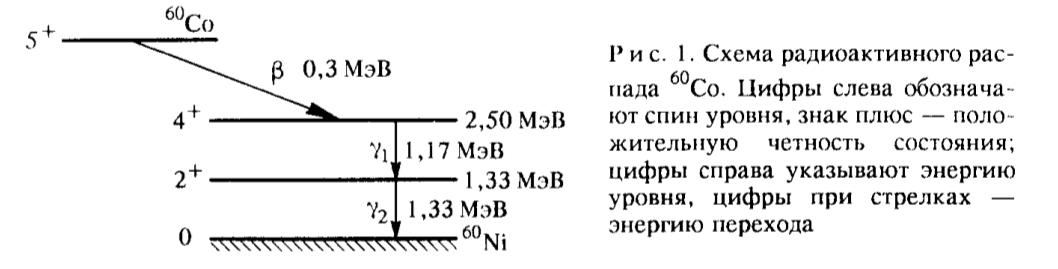
\includegraphics[width=0.7\linewidth]{picture.png}}
      \end{minipage}
      \label{pic:cobalt}
    \end{figure}

    Вероятность регистрации $\gamma$-кванта первым и вторым счетчиками:

    $$
      P_1=\frac{\omega _1 \varepsilon _1}{4 \pi}; \hspace{1cm}
      P_2=\frac{\omega _2 \varepsilon _2}{4 \pi}
    $$

    Если включить оба счетчика в сему совпадений с разрешающим временем
    $\tau >> 10^{-11}$с, то каскадные $\gamma$-кванты будут регистрироваться
    одновременно. Вероятность совпадения будет равна:

    $$
      P_{co}=P_1P_2
    $$

    Эта формула справедлива, если попадание одного $\gamma$-кванта  в первый
    счетчик и попадание второго во второй являются независимыми событиями.

    Вероятность истинных совпадений:

    $$
      P_{co}=W(\theta)P_1P_2
    $$

    где $W(\theta)$ - корреляционная функция, определяющая анизотропию
    направления вылета второго $\gamma$-кванта по отношению к направлению
    первого. При $\theta = 180^{\circ}$ для $^{60}Co$ $W=1.08$

    Получаем для абсолютной активности выражение:

    $$
      N_0=1.08 \frac{N_1N_2}{2N_{co}}
    $$

    где $N_1, N_2$ -истинные скорости счета, которые определяются как разность
    полной скорости счета и фона для каждого счетчика, а скорость истинных
    совпадений $N_{co}$ определяется как разность полного числа совпадений и
    числа случайных совпадений:

    $$
      n_c = 2 \tau n_1 n_2
    $$

    где $\tau$ - разрешающее время схемы совпадений.


  \section{Определение времени измерения}

    Определим какое время необходимо производить измерения, для того чтобы
    добиться заданной погрешности. Для этого дважды замерим скорость счета фона
    и излучения в течение минуты и выясним, какую погрешность имеет минутное
    измерение.

    Для закрытых ФЭУ нам необходимо добиться погрешности $1 \%$. Так, составим
    таблицу. \\

    \begin{tabular}{ || c || c | c | c ||}
      \hline
      Устройство & $N_{1ф}$ & $N_{2ф}$ & $\varepsilon_N$ \\ \hline
      ФЭУ$_1$ & $5527$ & $5440$ & $1.59 \%$ \\
      ФЭУ$_2$ & $2393$ & $2443$ & $2.07 \%$ \\
      \hline
    \end{tabular} \\

    Таким же образом построим таблицу для открытых ФЭУ. Для открытых ФЭУ
    необходимо добиться погрешности $0.5 \%$ \\

    \begin{tabular}{ || c || c | c | c ||}
      \hline
      Устройство & $N_{1ф}$ & $N_{2ф}$ & $\varepsilon_N$ \\ \hline
      ФЭУ$_1$ & $311463$ & $314004$ & $0.81 \%$ \\
      ФЭУ$_2$ & $160015$ & $158823$ & $0.75 \%$ \\
      \hline
    \end{tabular} \\

    Так, для получения необходимой погрешности необходимо производить измерения
    в течение следующих времен: для открытого и закрытого ФЭУ$_1$ -- $3$ минуты,
    для открытого ФЭУ$_2$ -- $3$ минуты, для закрытого -- $5$ минут.


  \section{Измерение скоростей счёта фона}

    \begin{tabular}{ || c || c | c | c ||}
      \hline
      Устройство & $t$, мин & $N_{ф}$ & $n_{ф}$, с$^{-1}$ \\ \hline
      ФЭУ$_1$ & $3$ & $17054$ & $94.74$ \\
      ФЭУ$_2$ & $5$ & $14081$ & $46.94$ \\
      \hline
    \end{tabular} \\


  \section{Измерение скоростей счёта излучения}

    Откроем ФЭУ и будем мерять скорость излучения в течение времени,
    необходимого для получения погрешности $0.5 \%$ \\

    \begin{tabular}{ || c || c | c | c ||}
      \hline
      Устройство & $t$, мин & $N_{п}$ & $n_{п}$, с$^{-1}$ \\ \hline
      ФЭУ$_1$ & $3$ & $959356$ & $5329.76$ \\
      ФЭУ$_2$ & $3$ & $484083$ & $2689.35$ \\
      \hline
    \end{tabular} \\


  \section{Измерение скоростей счета совпадений}

    Измерим скорость счета в режиме совпадений. В этом режиме мы будем считать
    количество совпадающих срабатываний обоих ФЭУ в рамках времени разрешающей
    способности.

    В данном случае выбрали длительность замера $4$ минуты. Так мы добьемся
    достаточно малой погрешности.

    Для подсчета $N_0$ воспользуемся формулой

    $$
      N_0 = 1.08 \frac{N_1 N_2}{2 N_{совп}} =
      1.08 \frac{\left(n_{1п} - n_{1ф}\right)\left(n_{2п} - n_{2ф}\right)}
      {2 \left(n_{совп} - 2 \tau n_{1п} n_{2п}\right)}
    $$ \\

    \begin{tabular}{ || c || c | c | c | c ||}
      \hline
      $\tau$, мкс & $t$, мин & $N_{совп}$ & $n_{совп}$, c$^{-1}$ & $N_0$, Бк \\
      \hline
      $0.2$ & $4$ & $1894$ & $7.89$ & $3461093$ \\
      $0.5$ & $4$ & $3951$ & $16.46$ & $3508749$ \\
      $1.0$ & $4$ & $7397$ & $30.82$ & $3468418$ \\
      \hline
    \end{tabular} \\

    Построим график зависимости скорости счёта от разрешающей способности.

    \begin{figure}[h!]
      \begin{minipage}[h]{0.6\linewidth}
        \center{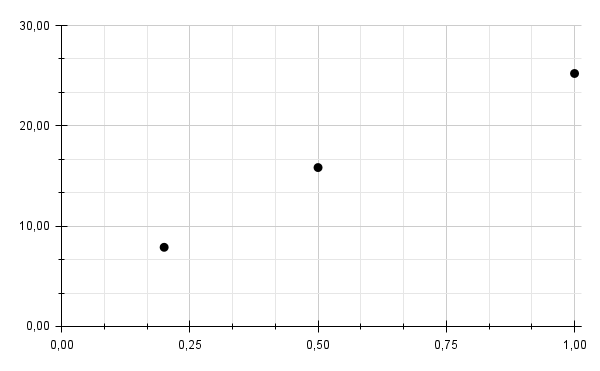
\includegraphics[width=\linewidth]{plot.png}}
      \end{minipage}
      \label{plot}
    \end{figure}

    Из графика можно понять, что абсолютная активность $^{60}Co$ составляет
    примерно $3.44$ МБк. Очевидно, что погрешность определения абсолютной
    активности заметно растет с увеличением разрешающей способности.

  \section{Вывод}

    В ходе проведения измерений получили абсолютную активность $^{60}Co$
    $N_0 \approx 3.44$ МБк и выяснили, что при увеличении разрешающей способности
    заметно растет неточность в определении абсолютной активности.

\end{document}
